\documentclass{article}\usepackage[]{graphicx}\usepackage[]{xcolor}
% maxwidth is the original width if it is less than linewidth
% otherwise use linewidth (to make sure the graphics do not exceed the margin)
\makeatletter
\def\maxwidth{ %
  \ifdim\Gin@nat@width>\linewidth
    \linewidth
  \else
    \Gin@nat@width
  \fi
}
\makeatother

\definecolor{fgcolor}{rgb}{0.345, 0.345, 0.345}
\newcommand{\hlnum}[1]{\textcolor[rgb]{0.686,0.059,0.569}{#1}}%
\newcommand{\hlstr}[1]{\textcolor[rgb]{0.192,0.494,0.8}{#1}}%
\newcommand{\hlcom}[1]{\textcolor[rgb]{0.678,0.584,0.686}{\textit{#1}}}%
\newcommand{\hlopt}[1]{\textcolor[rgb]{0,0,0}{#1}}%
\newcommand{\hlstd}[1]{\textcolor[rgb]{0.345,0.345,0.345}{#1}}%
\newcommand{\hlkwa}[1]{\textcolor[rgb]{0.161,0.373,0.58}{\textbf{#1}}}%
\newcommand{\hlkwb}[1]{\textcolor[rgb]{0.69,0.353,0.396}{#1}}%
\newcommand{\hlkwc}[1]{\textcolor[rgb]{0.333,0.667,0.333}{#1}}%
\newcommand{\hlkwd}[1]{\textcolor[rgb]{0.737,0.353,0.396}{\textbf{#1}}}%
\let\hlipl\hlkwb

\usepackage{framed}
\makeatletter
\newenvironment{kframe}{%
 \def\at@end@of@kframe{}%
 \ifinner\ifhmode%
  \def\at@end@of@kframe{\end{minipage}}%
  \begin{minipage}{\columnwidth}%
 \fi\fi%
 \def\FrameCommand##1{\hskip\@totalleftmargin \hskip-\fboxsep
 \colorbox{shadecolor}{##1}\hskip-\fboxsep
     % There is no \\@totalrightmargin, so:
     \hskip-\linewidth \hskip-\@totalleftmargin \hskip\columnwidth}%
 \MakeFramed {\advance\hsize-\width
   \@totalleftmargin\z@ \linewidth\hsize
   \@setminipage}}%
 {\par\unskip\endMakeFramed%
 \at@end@of@kframe}
\makeatother

\definecolor{shadecolor}{rgb}{.97, .97, .97}
\definecolor{messagecolor}{rgb}{0, 0, 0}
\definecolor{warningcolor}{rgb}{1, 0, 1}
\definecolor{errorcolor}{rgb}{1, 0, 0}
\newenvironment{knitrout}{}{} % an empty environment to be redefined in TeX

\usepackage{alltt}
\usepackage[sc]{mathpazo}
\renewcommand{\sfdefault}{lmss}
\renewcommand{\ttdefault}{lmtt}
\usepackage[T1]{fontenc}
\usepackage{geometry}
\geometry{verbose,tmargin=2.5cm,bmargin=2.5cm,lmargin=2.5cm,rmargin=2.5cm}
\setcounter{secnumdepth}{2}
\setcounter{tocdepth}{2}
\usepackage[unicode=true,pdfusetitle,
 bookmarks=true,bookmarksnumbered=true,bookmarksopen=true,bookmarksopenlevel=2,
 breaklinks=false,pdfborder={0 0 1},backref=false,colorlinks=false]
 {hyperref}
\hypersetup{
 pdfstartview={XYZ null null 1}}

\makeatletter
%%%%%%%%%%%%%%%%%%%%%%%%%%%%%% User specified LaTeX commands.
\renewcommand{\textfraction}{0.05}
\renewcommand{\topfraction}{0.8}
\renewcommand{\bottomfraction}{0.8}
\renewcommand{\floatpagefraction}{0.75}

\makeatother
\IfFileExists{upquote.sty}{\usepackage{upquote}}{}
\begin{document}



\title{\title{\title{\title{\title{\title{\title{\title{\title{\title{\title{}}}}}}}}}}}



\maketitle
The results below are generated from an R script.

\begin{knitrout}
\definecolor{shadecolor}{rgb}{0.969, 0.969, 0.969}\color{fgcolor}\begin{kframe}
\begin{alltt}
\hlcom{# 1. Lectura y preparación de datos}

\hlcom{# Lectura de datos}
\hlcom{# Strings como factores}
\hlkwd{library}\hlstd{(readr)}
\hlkwd{library}\hlstd{(Hmisc)}
\hlstd{ACMETelephoneABT} \hlkwb{<-} \hlkwd{read_csv}\hlstd{(}\hlstr{"./datos/ACMETelephoneABT.csv"}\hlstd{,} \hlkwc{na} \hlstd{=} \hlkwd{c}\hlstd{(}\hlstr{""}\hlstd{,} \hlstr{" "}\hlstd{))}
\end{alltt}


{\ttfamily\noindent\itshape\color{messagecolor}{\#\# Rows: 10000 Columns: 33\\\#\# -- Column specification ------------------------------------------------------------------\\\#\# Delimiter: "{},"{}\\\#\# chr \ (5): occupation, regionType, marriageStatus, creditRating, creditCard\\\#\# dbl (24): customer, age, income, numHandsets, handsetAge, currentHandsetPrice, avgBill...\\\#\# lgl \ (4): children, smartPhone, homeOwner, churn\\\#\# \\\#\# i Use `spec()` to retrieve the full column specification for this data.\\\#\# i Specify the column types or set `show\_col\_types = FALSE` to quiet this message.}}\begin{alltt}
\hlcom{# Corregir NAs y unificar valores en regionType}
\hlstd{ACMETelephoneABT}\hlopt{$}\hlstd{regionType[}\hlkwd{which}\hlstd{(ACMETelephoneABT}\hlopt{$}\hlstd{regionType} \hlopt{==} \hlstr{"unknown"}\hlstd{)]} \hlkwb{<-} \hlnum{NA}
\hlstd{ACMETelephoneABT}\hlopt{$}\hlstd{regionType[}\hlkwd{which}\hlstd{(ACMETelephoneABT}\hlopt{$}\hlstd{regionType} \hlopt{==} \hlstr{"r"}\hlstd{)]} \hlkwb{<-} \hlstr{"RURAL"}
\hlstd{ACMETelephoneABT}\hlopt{$}\hlstd{regionType[}\hlkwd{which}\hlstd{(ACMETelephoneABT}\hlopt{$}\hlstd{regionType} \hlopt{==} \hlstr{"s"}\hlstd{)]} \hlkwb{<-} \hlstr{"SUBURBAN"}
\hlstd{ACMETelephoneABT}\hlopt{$}\hlstd{regionType[}\hlkwd{which}\hlstd{(ACMETelephoneABT}\hlopt{$}\hlstd{regionType} \hlopt{==} \hlstr{"t"}\hlstd{)]} \hlkwb{<-} \hlstr{"TOWN"}
\hlstd{ACMETelephoneABT}\hlopt{$}\hlstd{regionType} \hlkwb{=} \hlkwd{factor}\hlstd{(ACMETelephoneABT}\hlopt{$}\hlstd{regionType,} \hlkwc{levels} \hlstd{=} \hlkwd{c}\hlstd{(}\hlstr{"RURAL"}\hlstd{,} \hlstr{"SUBURBAN"}\hlstd{,} \hlstr{"TOWN"}\hlstd{))}

\hlcom{# Corregir NAs en marriageStatus}
\hlstd{ACMETelephoneABT}\hlopt{$}\hlstd{marriageStatus[}\hlkwd{which}\hlstd{(ACMETelephoneABT}\hlopt{$}\hlstd{marriageStatus} \hlopt{==} \hlstr{"unknown"}\hlstd{)]} \hlkwb{<-} \hlnum{NA}
\hlstd{ACMETelephoneABT}\hlopt{$}\hlstd{marriageStatus} \hlkwb{=} \hlkwd{factor}\hlstd{(ACMETelephoneABT}\hlopt{$}\hlstd{marriageStatus,} \hlkwc{levels} \hlstd{=} \hlkwd{c}\hlstd{(}\hlstr{"YES"}\hlstd{,} \hlstr{"NO"}\hlstd{))}

\hlcom{# Corregir NAs y unificar valores en creditCard}
\hlstd{ACMETelephoneABT}\hlopt{$}\hlstd{creditCard[}\hlkwd{which}\hlstd{(ACMETelephoneABT}\hlopt{$}\hlstd{creditCard} \hlopt{==} \hlstr{"f"}\hlstd{)]} \hlkwb{<-} \hlstr{"FALSE"}
\hlstd{ACMETelephoneABT}\hlopt{$}\hlstd{creditCard[}\hlkwd{which}\hlstd{(ACMETelephoneABT}\hlopt{$}\hlstd{creditCard} \hlopt{==} \hlstr{"no"}\hlstd{)]} \hlkwb{<-} \hlstr{"FALSE"}
\hlstd{ACMETelephoneABT}\hlopt{$}\hlstd{creditCard[}\hlkwd{which}\hlstd{(ACMETelephoneABT}\hlopt{$}\hlstd{creditCard} \hlopt{==} \hlstr{"t"}\hlstd{)]} \hlkwb{<-} \hlstr{"TRUE"}
\hlstd{ACMETelephoneABT}\hlopt{$}\hlstd{creditCard[}\hlkwd{which}\hlstd{(ACMETelephoneABT}\hlopt{$}\hlstd{creditCard} \hlopt{==} \hlstr{"yes"}\hlstd{)]} \hlkwb{<-} \hlstr{"TRUE"}
\hlstd{ACMETelephoneABT}\hlopt{$}\hlstd{creditCard} \hlkwb{=} \hlkwd{factor}\hlstd{(ACMETelephoneABT}\hlopt{$}\hlstd{creditCard,} \hlkwc{levels} \hlstd{=} \hlkwd{c}\hlstd{(}\hlstr{"TRUE"}\hlstd{,} \hlstr{"FALSE"}\hlstd{))}

\hlcom{# Asignar NAs a casos con edad = 0}
\hlstd{ACMETelephoneABT}\hlopt{$}\hlstd{age[}\hlkwd{which}\hlstd{(ACMETelephoneABT}\hlopt{$}\hlstd{age} \hlopt{==} \hlnum{0}\hlstd{)]} \hlkwb{<-} \hlnum{NA}

\hlcom{# Asumimos casos de income = 0 como NAs}
\hlstd{ACMETelephoneABT}\hlopt{$}\hlstd{income[}\hlkwd{which}\hlstd{(ACMETelephoneABT}\hlopt{$}\hlstd{income} \hlopt{==} \hlnum{0}\hlstd{)]} \hlkwb{<-} \hlnum{NA}

\hlkwd{levels}\hlstd{(ACMETelephoneABT}\hlopt{$}\hlstd{creditCard)}
\end{alltt}
\begin{verbatim}
## [1] "TRUE"  "FALSE"
\end{verbatim}
\begin{alltt}
\hlkwd{levels}\hlstd{(ACMETelephoneABT}\hlopt{$}\hlstd{regionType)}
\end{alltt}
\begin{verbatim}
## [1] "RURAL"    "SUBURBAN" "TOWN"
\end{verbatim}
\begin{alltt}
\hlkwd{levels}\hlstd{(ACMETelephoneABT}\hlopt{$}\hlstd{marriageStatus)}
\end{alltt}
\begin{verbatim}
## [1] "YES" "NO"
\end{verbatim}
\begin{alltt}
\hlstd{ACMETelephoneABT}\hlopt{$}\hlstd{churn} \hlkwb{=} \hlkwd{ifelse}\hlstd{(ACMETelephoneABT}\hlopt{$}\hlstd{churn} \hlopt{==} \hlstr{"TRUE"}\hlstd{,} \hlnum{1}\hlstd{,} \hlnum{0}\hlstd{)}
\hlstd{ACMETelephoneABT}\hlopt{$}\hlstd{churn} \hlkwb{=} \hlkwd{factor}\hlstd{(ACMETelephoneABT}\hlopt{$}\hlstd{churn,} \hlkwc{levels} \hlstd{=} \hlkwd{c}\hlstd{(}\hlnum{1}\hlstd{,}\hlnum{0}\hlstd{))}
\hlkwd{summary}\hlstd{(ACMETelephoneABT}\hlopt{$}\hlstd{churn)}
\end{alltt}
\begin{verbatim}
##    1    0 
## 5000 5000
\end{verbatim}
\begin{alltt}
\hlkwd{levels}\hlstd{(ACMETelephoneABT}\hlopt{$}\hlstd{churn)}
\end{alltt}
\begin{verbatim}
## [1] "1" "0"
\end{verbatim}
\begin{alltt}
\hlcom{# 2. División de datos}
\hlkwd{library}\hlstd{(caret)}
\hlkwd{library}\hlstd{(dplyr)}

\hlkwd{set.seed}\hlstd{(}\hlnum{12345}\hlstd{)}
\hlstd{inTraining} \hlkwb{<-} \hlkwd{createDataPartition}\hlstd{(}\hlkwd{pull}\hlstd{(ACMETelephoneABT, churn),}
                                  \hlkwc{p} \hlstd{=} \hlnum{.7}\hlstd{,} \hlkwc{list} \hlstd{=} \hlnum{FALSE}\hlstd{,} \hlkwc{times} \hlstd{=} \hlnum{1}\hlstd{)}
\hlstd{acme_training} \hlkwb{<-} \hlkwd{slice}\hlstd{(ACMETelephoneABT, inTraining)}
\hlstd{acme_testing} \hlkwb{<-} \hlkwd{slice}\hlstd{(ACMETelephoneABT,} \hlopt{-}\hlstd{inTraining)}

\hlcom{# 3. Modelo 1. Regresión Logística}
\hlstd{min_overbundlemins} \hlkwb{=} \hlkwd{min}\hlstd{(acme_training}\hlopt{$}\hlstd{avgOverBundleMins)}
\hlstd{min_handsetAge} \hlkwb{=} \hlkwd{min}\hlstd{(acme_training}\hlopt{$}\hlstd{handsetAge)}
\hlstd{acme_training} \hlkwb{<-} \hlstd{acme_training} \hlopt
  \hlkwd{mutate}\hlstd{(}\hlkwc{binary_billAmountChangePct} \hlstd{=} \hlkwd{ifelse}\hlstd{(billAmountChangePct} \hlopt{>} \hlnum{0}\hlstd{,} \hlstr{"positive"}\hlstd{,}\hlstr{"negative"}\hlstd{))}
\hlstd{acme_training} \hlkwb{<-} \hlstd{acme_training} \hlopt
  \hlkwd{mutate}\hlstd{(}\hlkwc{creditRating_DE} \hlstd{=} \hlkwd{ifelse}\hlstd{(creditRating} \hlopt \hlkwd{c}\hlstd{(}\hlstr{"D"}\hlstd{,} \hlstr{"E"}\hlstd{),} \hlstr{"yes"}\hlstd{,}\hlstr{"no"}\hlstd{))}
\hlstd{acme_training}\hlopt{$}\hlstd{creditRating_DE} \hlkwb{=} \hlkwd{as.factor}\hlstd{(acme_training}\hlopt{$}\hlstd{creditRating_DE )}

\hlstd{acme_training}\hlopt{$}\hlstd{creditRating} \hlkwb{=} \hlkwd{as.factor}\hlstd{(acme_training}\hlopt{$}\hlstd{creditRating)}
\hlstd{acme_training}\hlopt{$}\hlstd{binary_billAmountChangePct} \hlkwb{=} \hlkwd{as.factor}\hlstd{(acme_training}\hlopt{$}\hlstd{binary_billAmountChangePct)}
\hlstd{acme_training}\hlopt{$}\hlstd{homeOwner} \hlkwb{=} \hlkwd{as.factor}\hlstd{(acme_training}\hlopt{$}\hlstd{homeOwner)}
\hlstd{acme_training}\hlopt{$}\hlstd{smartPhone} \hlkwb{=} \hlkwd{as.factor}\hlstd{(acme_training}\hlopt{$}\hlstd{smartPhone)}

\hlstd{glm_model_train} \hlkwb{=} \hlkwd{glm}\hlstd{(churn} \hlopt{~}
                        \hlkwd{log}\hlstd{(lastMonthCustomerCareCalls} \hlopt{+} \hlnum{1}\hlstd{)} \hlopt{+}
                        \hlkwd{log}\hlstd{(avgrecurringCharge} \hlopt{+} \hlnum{1}\hlstd{)} \hlopt{+} \hlkwd{log}\hlstd{(peakOffPeakRatio} \hlopt{+} \hlnum{1}\hlstd{)} \hlopt{+}
                        \hlkwd{log}\hlstd{(avgBill} \hlopt{+} \hlnum{1}\hlstd{)} \hlopt{+} \hlkwd{log}\hlstd{(avgReceivedMins} \hlopt{+} \hlnum{1}\hlstd{)} \hlopt{+}
                        \hlstd{creditRating_DE} \hlopt{+} \hlstd{binary_billAmountChangePct} \hlopt{+} \hlstd{smartPhone,}
                      \hlkwc{data}\hlstd{=acme_training,} \hlkwc{family}\hlstd{= binomial)}
\hlkwd{summary}\hlstd{(glm_model_train)}
\end{alltt}
\begin{verbatim}
## 
## Call:
## glm(formula = churn ~ log(lastMonthCustomerCareCalls + 1) + log(avgrecurringCharge + 
##     1) + log(peakOffPeakRatio + 1) + log(avgBill + 1) + log(avgReceivedMins + 
##     1) + creditRating_DE + binary_billAmountChangePct + smartPhone, 
##     family = binomial, data = acme_training)
## 
## Coefficients:
##                                     Estimate Std. Error z value Pr(>|z|)    
## (Intercept)                         -1.03816    0.17953  -5.783 7.36e-09 ***
## log(lastMonthCustomerCareCalls + 1)  0.10947    0.03471   3.154  0.00161 ** 
## log(avgrecurringCharge + 1)          0.49064    0.06612   7.421 1.16e-13 ***
## log(peakOffPeakRatio + 1)            0.06740    0.04217   1.598  0.10997    
## log(avgBill + 1)                    -0.39265    0.06696  -5.864 4.52e-09 ***
## log(avgReceivedMins + 1)             0.02763    0.01592   1.735  0.08273 .  
## creditRating_DEyes                   0.24202    0.06106   3.964 7.38e-05 ***
## binary_billAmountChangePctpositive   0.11028    0.05200   2.121  0.03394 *  
## smartPhoneTRUE                       0.48571    0.08493   5.719 1.07e-08 ***
## ---
## Signif. codes:  0 '***' 0.001 '**' 0.01 '*' 0.05 '.' 0.1 ' ' 1
## 
## (Dispersion parameter for binomial family taken to be 1)
## 
##     Null deviance: 9704.1  on 6999  degrees of freedom
## Residual deviance: 9542.9  on 6991  degrees of freedom
## AIC: 9560.9
## 
## Number of Fisher Scoring iterations: 4
\end{verbatim}
\begin{alltt}
\hlcom{# 3.1. Predicción sobre datos de test. Evaluación del modelo}
\hlstd{min_overbundlemins} \hlkwb{=} \hlkwd{min}\hlstd{(acme_testing}\hlopt{$}\hlstd{avgOverBundleMins)}
\hlstd{min_handsetAge} \hlkwb{=} \hlkwd{min}\hlstd{(acme_testing}\hlopt{$}\hlstd{handsetAge)}
\hlstd{acme_testing} \hlkwb{<-} \hlstd{acme_testing} \hlopt
  \hlkwd{mutate}\hlstd{(}\hlkwc{binary_billAmountChangePct} \hlstd{=} \hlkwd{ifelse}\hlstd{(billAmountChangePct} \hlopt{>} \hlnum{0}\hlstd{,} \hlstr{"positive"}\hlstd{,}\hlstr{"negative"}\hlstd{))}

\hlstd{acme_testing}\hlopt{$}\hlstd{income} \hlkwb{=} \hlkwd{as.factor}\hlstd{(acme_testing}\hlopt{$}\hlstd{income)}
\hlstd{acme_testing}\hlopt{$}\hlstd{binary_billAmountChangePct} \hlkwb{=} \hlkwd{as.factor}\hlstd{(acme_testing}\hlopt{$}\hlstd{binary_billAmountChangePct)}
\hlstd{acme_testing}\hlopt{$}\hlstd{homeOwner} \hlkwb{=} \hlkwd{as.factor}\hlstd{(acme_testing}\hlopt{$}\hlstd{homeOwner)}
\hlstd{acme_testing}\hlopt{$}\hlstd{smartPhone} \hlkwb{=} \hlkwd{as.factor}\hlstd{(acme_testing}\hlopt{$}\hlstd{smartPhone)}
\hlstd{acme_testing} \hlkwb{<-} \hlstd{acme_testing} \hlopt
  \hlkwd{mutate}\hlstd{(}\hlkwc{creditRating_DE} \hlstd{=} \hlkwd{ifelse}\hlstd{(creditRating} \hlopt \hlkwd{c}\hlstd{(}\hlstr{"D"}\hlstd{,} \hlstr{"E"}\hlstd{),} \hlstr{"yes"}\hlstd{,}\hlstr{"no"}\hlstd{))}
\hlstd{acme_testing}\hlopt{$}\hlstd{creditRating_DE} \hlkwb{=} \hlkwd{as.factor}\hlstd{(acme_testing}\hlopt{$}\hlstd{creditRating_DE )}

\hlstd{glm_probs} \hlkwb{=} \hlkwd{predict}\hlstd{(glm_model_train,} \hlkwc{newdata} \hlstd{= acme_testing,} \hlkwc{type} \hlstd{=} \hlstr{"response"}\hlstd{)}

\hlstd{umbral_dec} \hlkwb{=} \hlnum{0.46}
\hlstd{glm_probs} \hlkwb{<-} \hlkwd{ifelse}\hlstd{(glm_probs} \hlopt{>=} \hlstd{umbral_dec,} \hlnum{1}\hlstd{,} \hlnum{0}\hlstd{)}
\hlstd{glm_probs} \hlkwb{<-} \hlkwd{factor}\hlstd{(glm_probs,} \hlkwc{levels} \hlstd{=} \hlkwd{c}\hlstd{(}\hlnum{1}\hlstd{,}\hlnum{0}\hlstd{))}

\hlstd{tabla_conf} \hlkwb{<-} \hlkwd{table}\hlstd{(glm_probs, acme_testing}\hlopt{$}\hlstd{churn)}
\hlstd{tabla_conf}
\end{alltt}
\begin{verbatim}
##          
## glm_probs    1    0
##         1 1075 1200
##         0  425  300
\end{verbatim}
\begin{alltt}
\hlstd{caret}\hlopt{::}\hlkwd{confusionMatrix}\hlstd{(tabla_conf,} \hlkwc{positive} \hlstd{=} \hlstr{'1'}\hlstd{)}
\end{alltt}
\begin{verbatim}
## Confusion Matrix and Statistics
## 
##          
## glm_probs    1    0
##         1 1075 1200
##         0  425  300
##                                           
##                Accuracy : 0.4583          
##                  95% CI : (0.4404, 0.4764)
##     No Information Rate : 0.5             
##     P-Value [Acc > NIR] : 1               
##                                           
##                   Kappa : -0.0833         
##                                           
##  Mcnemar's Test P-Value : <2e-16          
##                                           
##             Sensitivity : 0.7167          
##             Specificity : 0.2000          
##          Pos Pred Value : 0.4725          
##          Neg Pred Value : 0.4138          
##              Prevalence : 0.5000          
##          Detection Rate : 0.3583          
##    Detection Prevalence : 0.7583          
##       Balanced Accuracy : 0.4583          
##                                           
##        'Positive' Class : 1               
## 
\end{verbatim}
\begin{alltt}
\hlcom{# Curva ROC}
\hlstd{logistic_gains_table} \hlkwb{<-} \hlkwd{blr_gains_table}\hlstd{(glm_model_train,} \hlkwc{data} \hlstd{= acme_testing)}
\hlkwd{blr_roc_curve}\hlstd{(logistic_gains_table)}
\end{alltt}
\end{kframe}

{\centering 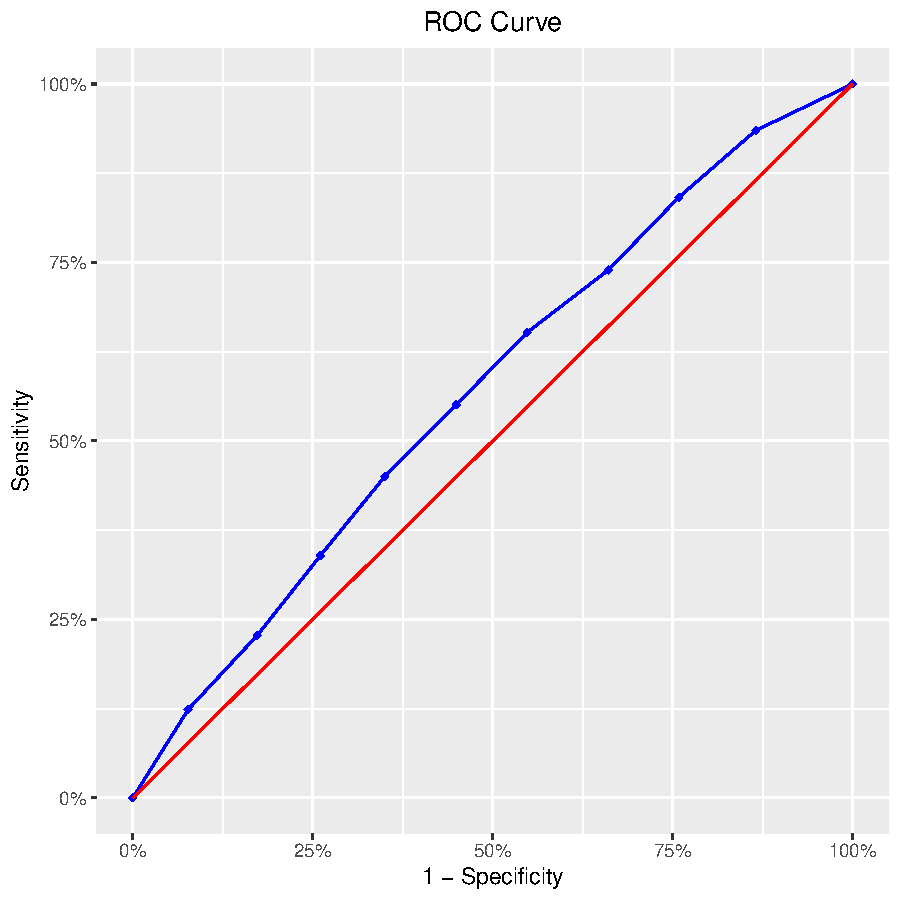
\includegraphics[width=.6\linewidth]{figure/RF1-SOLUCION-Rnwauto-report-1} 

}


\begin{kframe}\begin{alltt}
\hlcom{# 4. Modelo 2. Árbol de decisión}
\hlkwd{library}\hlstd{(partykit)}
\hlstd{ctree_acme} \hlkwb{=} \hlkwd{ctree}\hlstd{(churn} \hlopt{~} \hlstd{avgOverBundleMins} \hlopt{+}
                     \hlstd{lastMonthCustomerCareCalls} \hlopt{+}
                     \hlstd{avgrecurringCharge} \hlopt{+} \hlstd{peakOffPeakRatio} \hlopt{+}
                     \hlstd{binary_billAmountChangePct} \hlopt{+} \hlstd{smartPhone,}
                   \hlkwc{data}\hlstd{=acme_training)}
\hlstd{ctree_acme}
\end{alltt}
\begin{verbatim}
## 
## Model formula:
## churn ~ avgOverBundleMins + lastMonthCustomerCareCalls + avgrecurringCharge + 
##     peakOffPeakRatio + binary_billAmountChangePct + smartPhone
## 
## Fitted party:
## [1] root
## |   [2] avgrecurringCharge <= 37.41
## |   |   [3] smartPhone in FALSE: 1 (n = 458, err = 35.4%)
## |   |   [4] smartPhone in TRUE: 1 (n = 2015, err = 44.8%)
## |   [5] avgrecurringCharge > 37.41
## |   |   [6] smartPhone in FALSE: 1 (n = 237, err = 40.9%)
## |   |   [7] smartPhone in TRUE
## |   |   |   [8] binary_billAmountChangePct in negative: 0 (n = 2764, err = 47.1%)
## |   |   |   [9] binary_billAmountChangePct in positive: 0 (n = 1526, err = 42.5%)
## 
## Number of inner nodes:    4
## Number of terminal nodes: 5
\end{verbatim}
\begin{alltt}
\hlkwd{plot}\hlstd{(ctree_acme,} \hlkwc{gp} \hlstd{=} \hlkwd{gpar}\hlstd{(}\hlkwc{fontsize} \hlstd{=} \hlnum{10}\hlstd{),}
     \hlkwc{inner_panel}\hlstd{=node_inner,}
     \hlkwc{ip_args}\hlstd{=}\hlkwd{list}\hlstd{(}
       \hlkwc{abbreviate} \hlstd{=} \hlnum{TRUE}\hlstd{,}
       \hlkwc{id} \hlstd{=} \hlnum{FALSE}\hlstd{)}
\hlstd{)}
\end{alltt}
\end{kframe}

{\centering 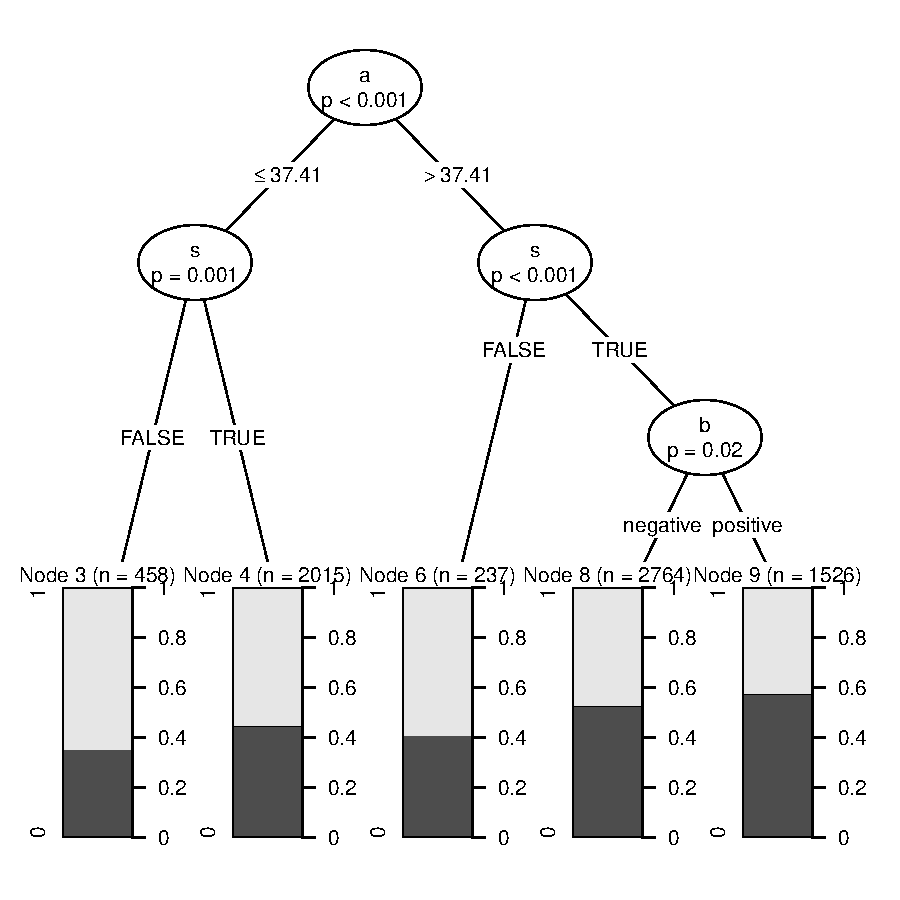
\includegraphics[width=.6\linewidth]{figure/RF1-SOLUCION-Rnwauto-report-2} 

}


\begin{kframe}\begin{alltt}
\hlkwd{library}\hlstd{(rpart)}
\hlkwd{library}\hlstd{(rpart.plot)}
\hlstd{rpart_acme} \hlkwb{=} \hlkwd{rpart}\hlstd{(churn} \hlopt{~} \hlstd{avgOverBundleMins} \hlopt{+}
                     \hlstd{lastMonthCustomerCareCalls} \hlopt{+}
                     \hlstd{avgrecurringCharge} \hlopt{+} \hlstd{peakOffPeakRatio} \hlopt{+}
                     \hlstd{binary_billAmountChangePct} \hlopt{+} \hlstd{smartPhone,}
                   \hlkwc{data}\hlstd{=acme_training)}
\hlstd{rpart_acme}
\end{alltt}
\begin{verbatim}
## n= 7000 
## 
## node), split, n, loss, yval, (yprob)
##       * denotes terminal node
## 
## 1) root 7000 3500 1 (0.5000000 0.5000000)  
##   2) avgrecurringCharge< 37.43 2473 1064 1 (0.5697533 0.4302467) *
##   3) avgrecurringCharge>=37.43 4527 2091 0 (0.4618953 0.5381047)  
##     6) smartPhone=FALSE 237   97 1 (0.5907173 0.4092827) *
##     7) smartPhone=TRUE 4290 1951 0 (0.4547786 0.5452214) *
\end{verbatim}
\begin{alltt}
\hlkwd{rpart.plot}\hlstd{(rpart_acme)}
\end{alltt}
\end{kframe}

{\centering 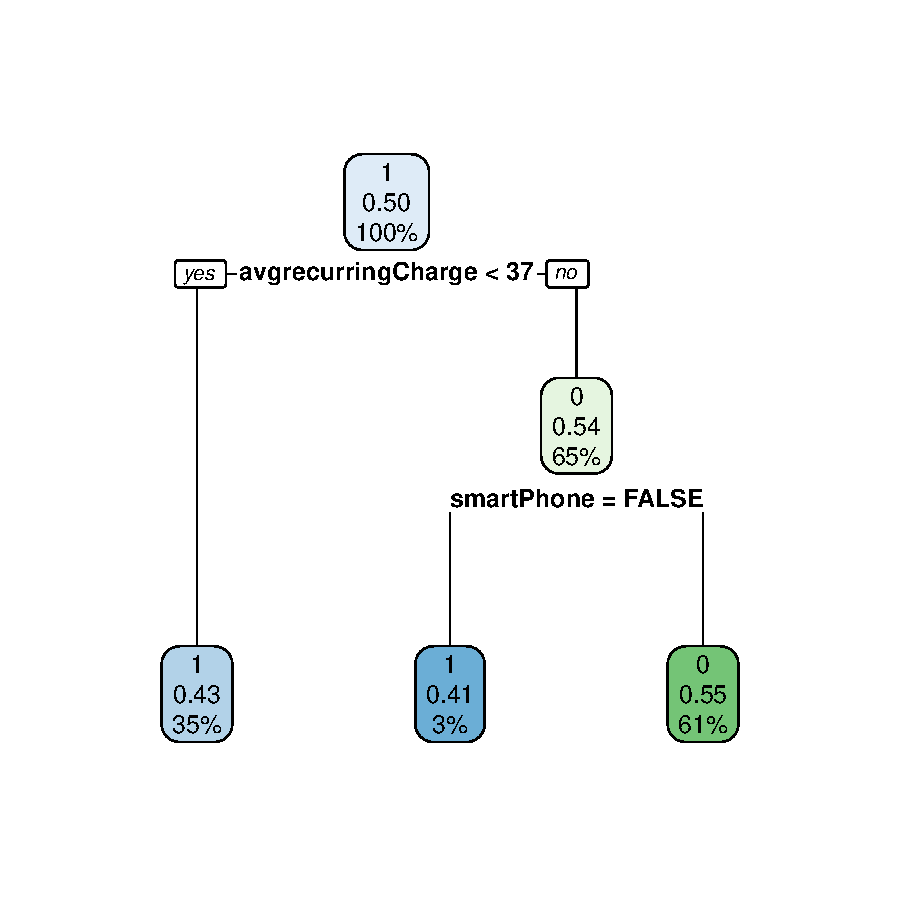
\includegraphics[width=.6\linewidth]{figure/RF1-SOLUCION-Rnwauto-report-3} 

}


\begin{kframe}\begin{alltt}
\hlcom{# 4.2 Predicción sobre datos de test}
\hlstd{ctree_pred} \hlkwb{<-} \hlkwd{predict}\hlstd{(ctree_acme,} \hlkwc{newdata}\hlstd{=acme_testing,} \hlkwc{type}\hlstd{=}\hlstr{'response'}\hlstd{)}
\hlkwd{confusionMatrix}\hlstd{(ctree_pred, acme_testing}\hlopt{$}\hlstd{churn)}
\end{alltt}
\begin{verbatim}
## Confusion Matrix and Statistics
## 
##           Reference
## Prediction   1   0
##          1 629 522
##          0 871 978
##                                           
##                Accuracy : 0.5357          
##                  95% CI : (0.5176, 0.5536)
##     No Information Rate : 0.5             
##     P-Value [Acc > NIR] : 5.005e-05       
##                                           
##                   Kappa : 0.0713          
##                                           
##  Mcnemar's Test P-Value : < 2.2e-16       
##                                           
##             Sensitivity : 0.4193          
##             Specificity : 0.6520          
##          Pos Pred Value : 0.5465          
##          Neg Pred Value : 0.5289          
##              Prevalence : 0.5000          
##          Detection Rate : 0.2097          
##    Detection Prevalence : 0.3837          
##       Balanced Accuracy : 0.5357          
##                                           
##        'Positive' Class : 1               
## 
\end{verbatim}
\begin{alltt}
\hlstd{rpart_pred} \hlkwb{<-} \hlkwd{predict}\hlstd{(rpart_acme,} \hlkwc{newdata}\hlstd{=acme_testing,} \hlkwc{type}\hlstd{=}\hlstr{'class'}\hlstd{)}
\hlkwd{confusionMatrix}\hlstd{(rpart_pred, acme_testing}\hlopt{$}\hlstd{churn)}
\end{alltt}
\begin{verbatim}
## Confusion Matrix and Statistics
## 
##           Reference
## Prediction   1   0
##          1 629 522
##          0 871 978
##                                           
##                Accuracy : 0.5357          
##                  95% CI : (0.5176, 0.5536)
##     No Information Rate : 0.5             
##     P-Value [Acc > NIR] : 5.005e-05       
##                                           
##                   Kappa : 0.0713          
##                                           
##  Mcnemar's Test P-Value : < 2.2e-16       
##                                           
##             Sensitivity : 0.4193          
##             Specificity : 0.6520          
##          Pos Pred Value : 0.5465          
##          Neg Pred Value : 0.5289          
##              Prevalence : 0.5000          
##          Detection Rate : 0.2097          
##    Detection Prevalence : 0.3837          
##       Balanced Accuracy : 0.5357          
##                                           
##        'Positive' Class : 1               
## 
\end{verbatim}
\begin{alltt}
\hlcom{# 5. Modelo 3: Random Forest}
\hlkwd{library}\hlstd{(randomForest)}

\hlstd{forest_acme} \hlkwb{=} \hlkwd{randomForest}\hlstd{(churn} \hlopt{~} \hlstd{avgOverBundleMins} \hlopt{+}
                             \hlstd{lastMonthCustomerCareCalls} \hlopt{+}
                             \hlstd{avgrecurringCharge} \hlopt{+} \hlstd{peakOffPeakRatio} \hlopt{+}
                             \hlstd{binary_billAmountChangePct} \hlopt{+} \hlstd{smartPhone,}
                           \hlkwc{data}\hlstd{=acme_training)}
\hlstd{forest_acme}
\end{alltt}
\begin{verbatim}
## 
## Call:
##  randomForest(formula = churn ~ avgOverBundleMins + lastMonthCustomerCareCalls +      avgrecurringCharge + peakOffPeakRatio + binary_billAmountChangePct +      smartPhone, data = acme_training) 
##                Type of random forest: classification
##                      Number of trees: 500
## No. of variables tried at each split: 2
## 
##         OOB estimate of  error rate: 45.7%
## Confusion matrix:
##      1    0 class.error
## 1 1797 1703   0.4865714
## 0 1496 2004   0.4274286
\end{verbatim}
\begin{alltt}
\hlkwd{library}\hlstd{(randomForestExplainer)}
\hlstd{importance_frame} \hlkwb{<-} \hlkwd{measure_importance}\hlstd{(forest_acme)}
\end{alltt}
\begin{verbatim}
## [1] "Warning: your forest does not contain information on local importance so 'accuracy_decrease' measure cannot be extracted. To add it regrow the forest with the option localImp = TRUE and run this function again."
\end{verbatim}
\begin{alltt}
\hlkwd{save}\hlstd{(importance_frame,} \hlkwc{file} \hlstd{=} \hlstr{"importance_frame.rda"}\hlstd{)}
\hlkwd{load}\hlstd{(}\hlstr{"importance_frame.rda"}\hlstd{)}
\hlkwd{plot_multi_way_importance}\hlstd{(importance_frame,} \hlkwc{size_measure} \hlstd{=} \hlstr{"no_of_nodes"}\hlstd{)}
\end{alltt}
\end{kframe}

{\centering 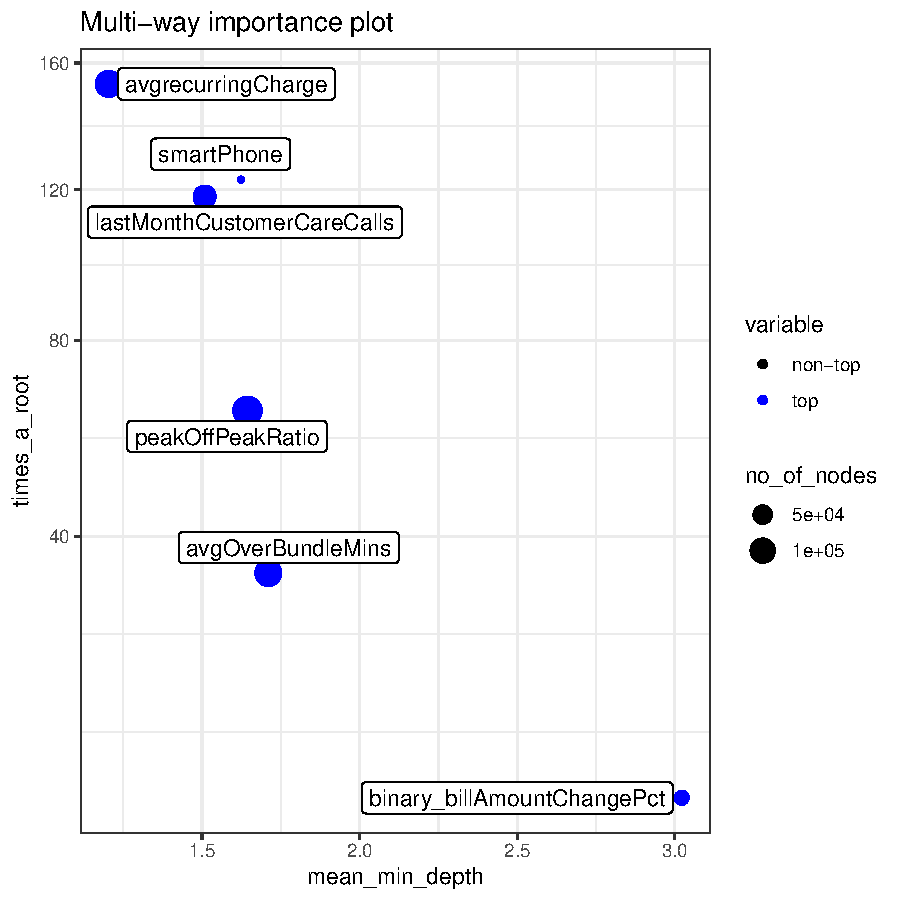
\includegraphics[width=.6\linewidth]{figure/RF1-SOLUCION-Rnwauto-report-4} 

}


\end{knitrout}

The R session information (including the OS info, R version and all
packages used):

\begin{knitrout}
\definecolor{shadecolor}{rgb}{0.969, 0.969, 0.969}\color{fgcolor}\begin{kframe}
\begin{alltt}
\hlkwd{sessionInfo}\hlstd{()}
\end{alltt}
\begin{verbatim}
## R version 4.3.1 (2023-06-16)
## Platform: x86_64-pc-linux-gnu (64-bit)
## Running under: Ubuntu 20.04.6 LTS
## 
## Matrix products: default
## BLAS:   /usr/lib/x86_64-linux-gnu/atlas/libblas.so.3.10.3 
## LAPACK: /usr/lib/x86_64-linux-gnu/atlas/liblapack.so.3.10.3;  LAPACK version 3.9.0
## 
## locale:
##  [1] LC_CTYPE=es_ES.UTF-8       LC_NUMERIC=C               LC_TIME=es_ES.UTF-8       
##  [4] LC_COLLATE=es_ES.UTF-8     LC_MONETARY=es_ES.UTF-8    LC_MESSAGES=es_ES.UTF-8   
##  [7] LC_PAPER=es_ES.UTF-8       LC_NAME=C                  LC_ADDRESS=C              
## [10] LC_TELEPHONE=C             LC_MEASUREMENT=es_ES.UTF-8 LC_IDENTIFICATION=C       
## 
## time zone: Europe/Madrid
## tzcode source: system (glibc)
## 
## attached base packages:
## [1] grid      stats     graphics  grDevices utils     datasets  methods   base     
## 
## other attached packages:
##  [1] randomForestExplainer_0.10.1 partykit_1.2-20             
##  [3] mvtnorm_1.2-3                libcoin_1.0-10              
##  [5] blorr_0.3.0                  Hmisc_5.1-1                 
##  [7] readr_2.1.4                  caretEnsemble_2.0.3         
##  [9] DALEX_2.4.3                  ROCR_1.0-11                 
## [11] randomForest_4.7-1.1         arulesViz_1.5-2             
## [13] arules_1.7-6                 Matrix_1.6-1.1              
## [15] liver_1.15                   ggfortify_0.4.16            
## [17] factoextra_1.0.7             mlbench_2.1-3.1             
## [19] readxl_1.4.3                 caret_6.0-94                
## [21] lattice_0.21-9               ggplot2_3.4.3               
## [23] rpart.plot_3.1.1             rpart_4.1.19                
## [25] caTools_1.18.2               dplyr_1.1.3                 
## [27] ISLR2_1.3-2                 
## 
## loaded via a namespace (and not attached):
##   [1] RColorBrewer_1.1-3   rstudioapi_0.15.0    jsonlite_1.8.7       magrittr_2.0.3      
##   [5] farver_2.1.1         rmarkdown_2.25       vctrs_0.6.3          base64enc_0.1-3     
##   [9] iBreakDown_2.0.1     tinytex_0.47         htmltools_0.5.6.1    cellranger_1.1.0    
##  [13] Formula_1.2-5        pROC_1.18.4          parallelly_1.36.0    htmlwidgets_1.6.2   
##  [17] plyr_1.8.9           lubridate_1.9.3      igraph_1.5.1         lifecycle_1.0.3     
##  [21] iterators_1.0.14     pkgconfig_2.0.3      R6_2.5.1             fastmap_1.1.1       
##  [25] future_1.33.0        digest_0.6.33        reshape_0.8.9        GGally_2.1.2        
##  [29] colorspace_2.1-0     labeling_0.4.3       fansi_1.0.5          timechange_0.2.0    
##  [33] abind_1.4-5          polyclip_1.10-6      compiler_4.3.1       proxy_0.4-27        
##  [37] bit64_4.0.5          withr_2.5.1          htmlTable_2.4.1      backports_1.4.1     
##  [41] carData_3.0-5        viridis_0.6.4        highr_0.10           ggforce_0.4.1       
##  [45] MASS_7.3-60          lava_1.7.2.1         ModelMetrics_1.2.2.2 tools_4.3.1         
##  [49] foreign_0.8-85       future.apply_1.11.0  nnet_7.3-19          glue_1.6.2          
##  [53] inum_1.0-5           nlme_3.1-163         checkmate_2.2.0      cluster_2.1.4       
##  [57] reshape2_1.4.4       generics_0.1.3       recipes_1.0.8        gtable_0.3.4        
##  [61] tzdb_0.4.0           class_7.3-22         tidyr_1.3.0          data.table_1.14.8   
##  [65] hms_1.1.3            car_3.1-2            tidygraph_1.2.3      utf8_1.2.3          
##  [69] ggrepel_0.9.3        foreach_1.5.2        pillar_1.9.0         stringr_1.5.0       
##  [73] vroom_1.6.4          splines_4.3.1        tweenr_2.0.2         survival_3.5-7      
##  [77] bit_4.0.5            tidyselect_1.2.0     pbapply_1.7-2        knitr_1.44          
##  [81] gridExtra_2.3        stats4_4.3.1         xfun_0.40            graphlayouts_1.0.1  
##  [85] hardhat_1.3.0        timeDate_4022.108    DT_0.30              visNetwork_2.1.2    
##  [89] stringi_1.7.12       yaml_2.3.7           evaluate_0.22        codetools_0.2-19    
##  [93] ggraph_2.1.0         tibble_3.2.1         cli_3.6.1            munsell_0.5.0       
##  [97] Rcpp_1.0.11          globals_0.16.2       parallel_4.3.1       ellipsis_0.3.2      
## [101] gower_1.0.1          bitops_1.0-7         listenv_0.9.0        viridisLite_0.4.2   
## [105] ipred_0.9-14         scales_1.2.1         prodlim_2023.08.28   e1071_1.7-13        
## [109] purrr_1.0.2          crayon_1.5.2         rlang_1.1.1
\end{verbatim}
\begin{alltt}
\hlkwd{Sys.time}\hlstd{()}
\end{alltt}
\begin{verbatim}
## [1] "2023-11-02 21:54:13 CET"
\end{verbatim}
\end{kframe}
\end{knitrout}


\end{document}
